\section{Implementação de Hardware}

\subsection{Sensor de Temperatura}

O sensor de temperatura DS18b20 é alimentado pelos pinos de 5V e GND (terra) do microcontrolador. seu sinal de leitura é enviado para uma porta digital, sendo utilizado um resistor de 4,7 k$\omega$ como pull up, caso exista uma leitura errada do sensor. A figura \ref{figura:micro_temp} ilustra a conexão do microcontrolador com o sensor de temperatura. 


\begin{figure}[h]
    \centering
    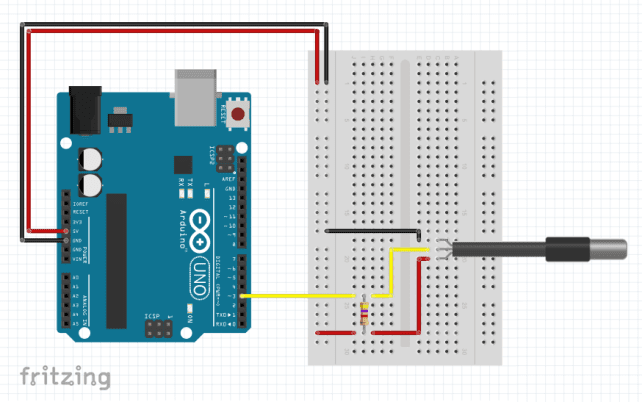
\includegraphics[scale=0.40]{figuras/implementacao/hardware/DSsensor.png}
    \caption{Esquema de conexão entre microcontrolador e sensor de temperatura DS18B20.}
    \label{fig:micro_temp}
\end{figure}


O excerto de código em linguagem Arduino a seguir representa a função utilizada para ler o valor de saída do sensor. A biblioteca OneWire (https://github.com/PaulStoffregen/OneWire) implementa o protocolo proprietário de comunicação serial da Dallas Semicondutor, fabricante do sensor. Ela é utilizada em conjunto com a biblioteca livre DallasTemperature (https://github.com/milesburton/Arduino-Temperature-Control-Library) para estabelecer a comunicação com o DS18B20.


% \begin{lstlisting}[language=C]

% #include <OneWire.h>
% #include <DallasTemperature.h>
% #define ONE_WIRE_BUS D6

% OneWire oneWire(ONE_WIRE_BUS);
% DallasTemperature sensors(&oneWire)

% void setup() {
%     sensors.begin();
% }

% float readTemperature() {
%     return sensors.getTempCByIndex(0);
% }

% \end{lstlisting}


\subsection{Sensor de pH}

O sensor de pH é conectado a um circuito auxiliar que trata o sinal proveniente da ponta de prova. Esse circuito é conectado aos pinos de 5V e GND do microcontrolador para alimentação, e envia do dado coletado por meio de sinal analógico, como observado na figura \ref{fig:micro_ph}. 


\begin{figure}[h]
    \centering
    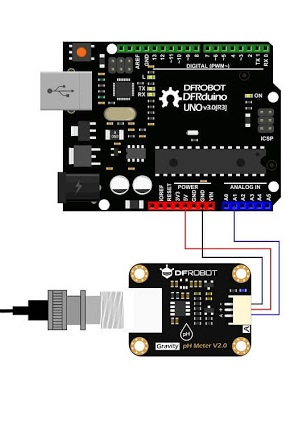
\includegraphics[scale=0.65]{figuras/implementacao/hardware/micro_ph.jpg}
    \caption{Esquema de conexão entre microcontrolador e sensor de pH E-201-C.}
    \label{fig:micro_ph}
\end{figure}


Para utilização desse sensor, é necessário sua calibração, que consiste na medição da tensão de saída do sensor em soluções com diferentes concentrações de \(H^+\) e obtenção de uma equação linear que traduza a voltagem medida em um valor de pH. Para isso utilizadas soluções tampão com pH iguais a 4, 7 e 10. A calibração seguiu o seguinte processo:
\begin{enumerate}
    \item Com a solução de pH igual a 7, ajustar o ganho do circuito (por um potenciômetro) até que a leitura de voltagem seja 2,5 Volts. Essa tensão foi escolhida de forma a coincidir valor médio da tensão de alimentação do circuito com o valor médio da escala de pH;
    \item Capturar a tensão medida nas soluções com pH 4 e 10;
    \item Aplicar regressão linear, minimizando a soma dos erros quadráticos, obtendo a reta que relaciona a tensão medida com o pH da solução
\end{enumerate}


Com os valores obtidos na tabela \ref{tab:calibra_ph}, foi obtida a equação linear \ref{eq:pH}.

\begin{equation}
    pH = 2.0171 * Voltagem + 1.7152
    \label{eq:pH}
\end{equation}


\begin{table}[H]
    \begin{center}
        \begin{tabular}{ |c|c| } 
            \hline
            Voltagem & pH \\
            \hline
            2.50 & 7.0 \\ 
            \hline
            1.20 & 4.0 \\ 
            \hline
            4.16 & 10.0 \\ 
            \hline
        \end{tabular}
        \caption{\label{tab:calibra_ph}Medições de tensão em soluções tampão para calibração do sensor de pH.}
    \end{center}
\end{table}


A leitura do pH medido pelo sensor pelo microcontrolador segue o seguinte algoritmo:
\begin{enumerate}
    \item Valor inteiro entre 0 e 1024 recebido pelo sensor é lido na porta analógica;
    \item Valor lido é convertido em uma diferença de tensão seguindo \(Voltagem = medida * 5 / 1024\);
    \item Diferença de tensão é convertida na leitura de pH seguindo equação linear obtida na calibração do sensor.
\end{enumerate}


% \begin{lstlisting}[language=C]

% int ph_pin = A0;

% float readPH() {
%     int measure = analogRead(ph_pin);
%     double voltage = measure * 5 / 1024;
%     return 2.0171 * voltage + 1.7152;
% }

% \end{lstlisting}


\subsection{Conexão e Comunicação do Microcontrolador}

Com os sensores propriamente conectados e calibrados, o microcontrolador foi configurado para se conectar à Internet através de conexão WiFi e a enviar os dados coletados por meio do protocolo MQTT. O Wemos D1 é controlada pelo módulo ESP8266, de forma que ofereça conectividade WiFi nativa. A biblioteca ESP8266WiFi (https://github.com/esp8266/Arduino/tree/master/libraries/ESP8266WiFi) foi utilizada para estabelecer a conexão Wifi, em conjunto com a biblioteca PubSubClient (https://github.com/knolleary/pubsubclient) para publicar mensagens e se inscrever em tópicos MQTT. 


% // TODO: Colocar código completo em Apêncice e discutir Fluxo completo aqui




